\documentclass[10pt]{acmsiggraph}               % final
%\documentclass[review]{acmsiggraph}      % review
%\documentclass[widereview]{acmsiggraph}  % wide-spaced review
%\documentclass[preprint]{acmsiggraph}    % preprint

%% Uncomment one of the four lines above depending on where your paper is
%% in the conference process. ``review'' and ``widereview'' are for review
%% submission, ``preprint'' is for pre-publication, and ``final'' is for
%% the version to be printed.

%% These two line bring in essential packages: ``mathptmx'' for Type 1 
%% typefaces, and ``graphicx'' for inclusion of EPS figures.

\usepackage{mathptmx}
\usepackage{graphicx}

%% use this for zero \parindent and non-zero \parskip, intelligently.

\usepackage{parskip}

\usepackage{amsmath}

%% If you are submitting a paper to the annual conference, please replace 
%% the value ``0'' below with your OnlineID. If you are not submitting this
%% paper to the annual conference, you may safely leave it at ``0'' -- it 
%% will not be included in the output.

\onlineid{0}

%% need to document this!

\acmformat{print}

%% Paper title.

\title{Segmenting Labeled Strokes\\
\small{July 2006}}

%% Author and Affiliation (single author).

\author{Devin Smith\\Harvey Mudd College\\dsmith@hmc.edu}%\thanks{e-mail: dsmith@hmc.edu}}


%% Keywords that describe your work.

\keywords{clustering, segmentation, sketch}

%%%%%% START OF THE PAPER %%%%%%

\begin{document}

%\teaser{
%	\includegraphics[width=1.5in]{SEGMENTATION.gif}%sample.eps}
%  \caption{Lookit! Lookit!}
%}

%% The ``\maketitle'' command must be the first command after the
%% ``\begin{document}'' command. It prepares and prints the title block.

\maketitle

\begin{abstract}
Sketching is a natural form of expressing a design.
Often we wish there was a way to automatically transform our sketch into a more final form.
Sketch recognition aims to alleviate this wish.
A part of sketch recognition involves a step called segmentation.
Segmentation consists of two steps: initial partitioning and updating partitioning.
Using label information for each stroke, we provide a method for initial partitioning and propose methods to update the partitioning in polynomial time.
\end{abstract}

\section{Problem Statement}

%% The ``\copyrightspace'' command must be the first command after the 
%% start of the first section of the body of your paper. It ensures the
%% copyright space is left at the bottom of the first column on the first
%% page of your paper.

%\copyrightspace

%\begin{itemize}
%\item What is a sketch?
%\item Why are we interested in sketches?
%\item Describe the overall problem we are trying to solve.
%\item Give concise problem that we are trying to solve with segmentation.
%\item Give overview of segmentation component and problem associated with that
%\item Note: Mention that with this segmentation we have more information than most
%do when they are segmenting. We have a label and probability for each stroke to
%supplement segmentation, while other approaches do not.
%\end{itemize}

%Feel I need to talk about the overall project here and what a sketch is.

Sketches are quick and simple ways to visually express a design.
Unfortunately, there are not many computer programs that can recognize a sketch.
Many of the programs that do exist place unnatural restrictions on how the user sketches, such as forcing the user to pause after every symbol has been drawn, imposing a single stroke to symbol correspondence, or imposing that multiple symbols cannot be made with a single stroke.
Our system aims to recognize digital logic diagram sketches, and implement the circuit in a simulator, without placing any restrictions on users' sketching styles.
 %What are some of the problems and difficulties in this domain?

Sketch recognition is more than just symbol recognition.
It usually consists of three main steps: preprocessing, segmentation, and symbol recognition.
Preprocessing takes a sketch and cleans up the data by removing unnecessary points and breaking up the strokes into lines and arcs.
Segmentation searches through the partitions of a sketch's strokes until it believes that each group in the partition represents a single component in the sketch.
Symbol recognition takes the parts from segmentation and tries to classify them.

In sketch recognition, segmentation, is the process of searching the partition space of a sketch.
The partition space of a sketch is the set of all possible partitions of the strokes within the sketch.
Searching the partition space consists of two steps: choosing an initial partition, and updating the current partition until the ``correct'' partition is found.
A ``correct'' partition is one where all parts of a sketch's segmentation can be recognized with some amount of certainty.
These parts are recognized with symbol recognition.
There is an intimate relationship between segmentation and symbol recognition.
The na\"{i}ve way to accomplish segmentation is to try every partition of the strokes.
While the na\"{i}ve way is simple to implement, it consumes exponential time.
This exponential time is why segmentation is arguably the most complex problem in sketch recognition~\cite{pattern}.
As a consequence, segmentation is rarely finished after a single element in the partition space has been tested.
Segmentation is a sequence trials and errors as it searches through the partition space.
For example, given a sketch composed of 20 strokes (a rather small sketch), there are more than 50 trillion elements in the partition space.
Our goal is to use the sketch data and domain specific information to segment a sketch in polynomial time.

For the logical circuit diagram domain, a correct partition would be a partition were there was a part for each component in the diagram.
The correct partition of Figure~\ref{fig:simple} is \{\{1\} \{2\} \{3 4\} \{5 6 7\} \{8\} \{9\} \{10 11\} \{12 13 14\} \{15 16\} \{17\}\}.
% with the corresponding recognition being AND:\{\{3 4\} \{15 16\}\}, OR:\{\{10 11\}\}, and WIRE:\{\{1\} \{2\} \{5 6 7\} \{8\} \{9\} \{12 13 14\} \{17\}\}. 
This partition may seem relatively trivial to find, yet consider that the strokes are unordered, overlapping, and inconsistent in size.

\begin{figure}[h]
\centering
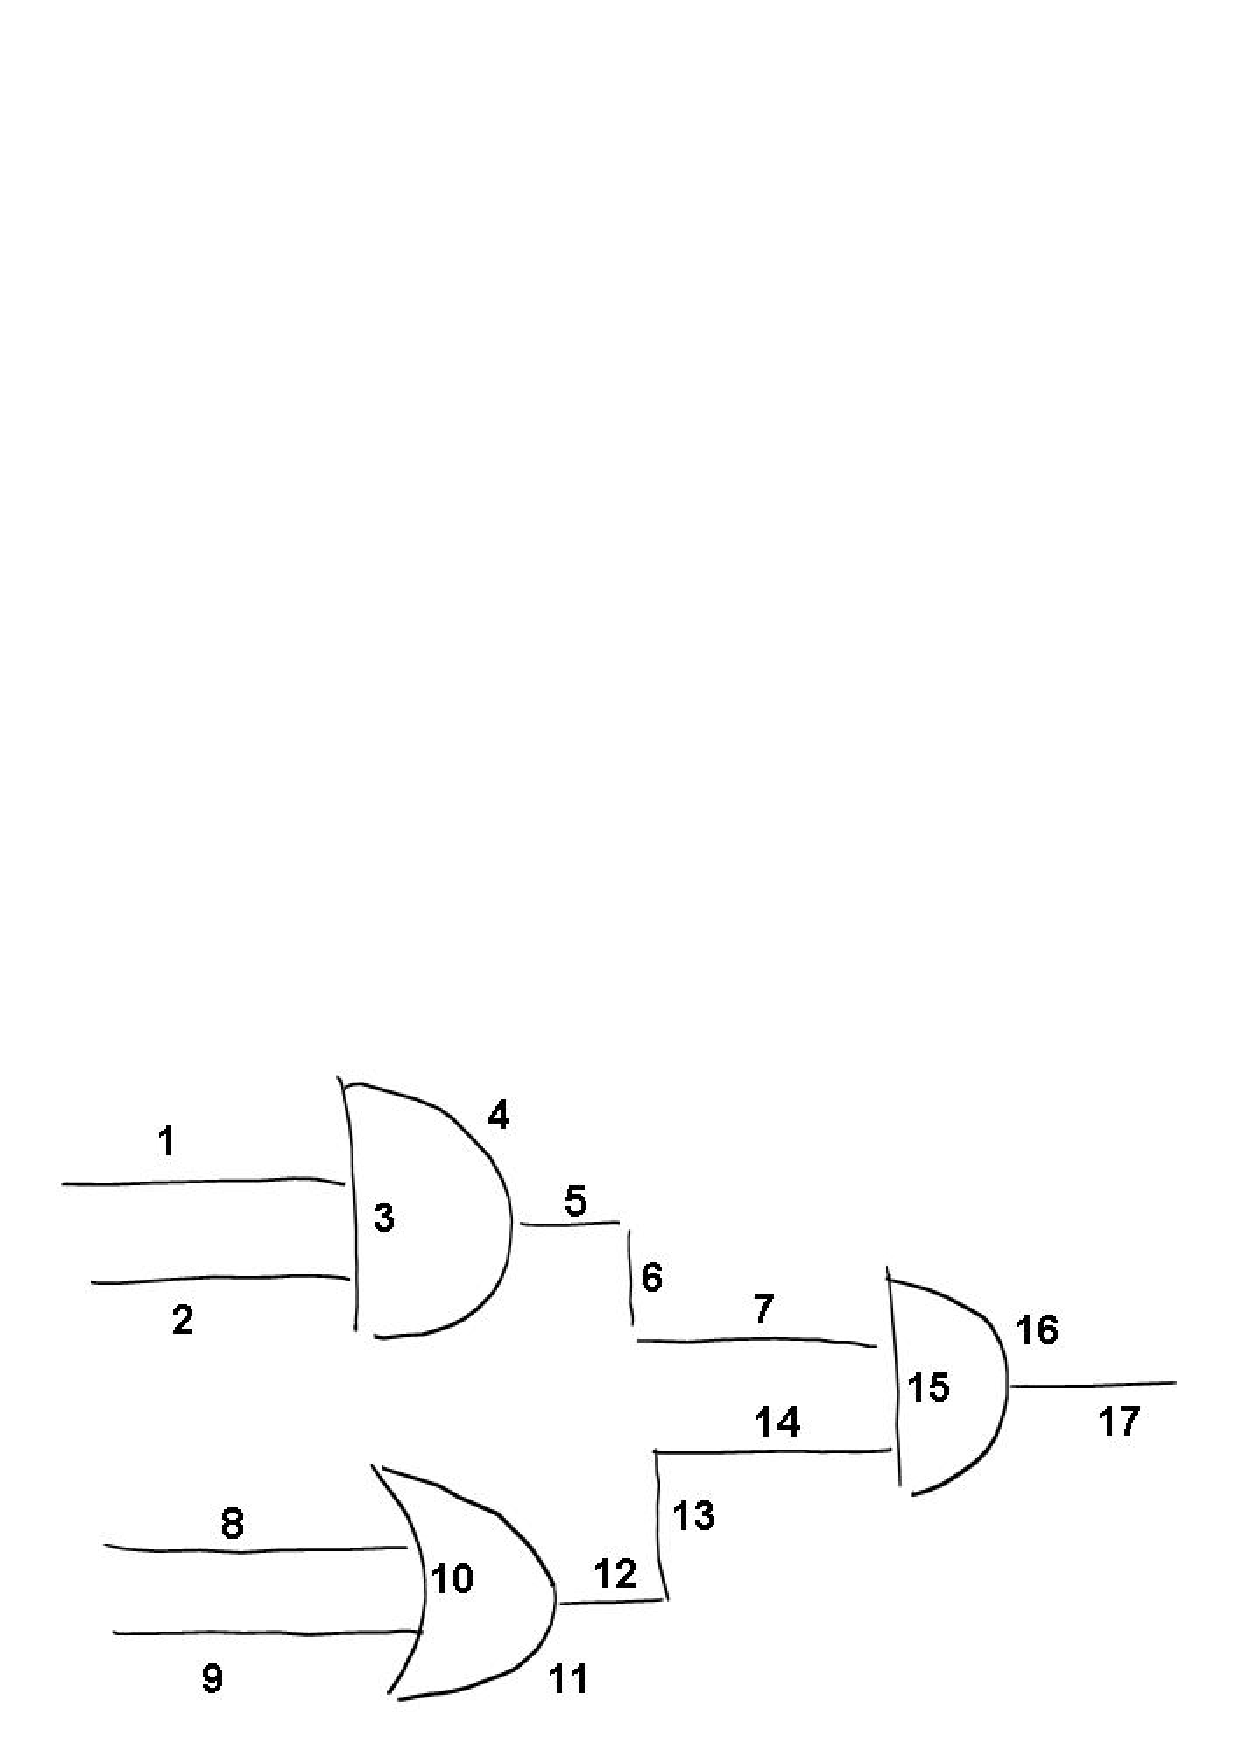
\includegraphics[width=3.0in]{nums.png}%sample.eps}
\caption{A Simple Digital Logic Diagram}
\label{fig:simple}
\end{figure}

In our system, we have an additional step in sketch recognition that makes our application of segmentation novel.
Before segmentation, the preprocessed sketch goes through a labeling step.
The labeling step applies a label and associated probability to each stroke in the sketch (see BLAH for implementation details... give reference).
For example, the labeling step may give stroke 1 the label ``WIRE'' with probability 95\%, and stroke 3 the label ``AND'' with probability 70\%.
Even though each stroke in the sketch now has a label, sketch recognition is \emph{not} done.
Sketch recognition is recognition of the sketch as a whole: that is, it recognizes all of the components and how they interconnect.
With only a label applied to each stroke, there is no sense of how the strokes fit together globally.
Sketch recognition is global recognition, while labeling is local recognition.

Even with this local recognition, segmentation is by no means trivial.
First of all, given the labeling ``AND'' to two strokes A and B with probabilities $X$ and $Y$, we cannot say that A and B are an ``AND'' gate with probability $X \times Y$ for three reasons: A and B are not independent, A and B may not belong to the same component, and A and B may not be the only strokes that compose the component.
Thus, to get the probability that A and B are an ``AND'' gate, we must use symbol recognition.
And while labels can help segmention, they can also hinder progress if they are wrong.
Segmentation should be able to take into account the labels, yet adjust them if they are wrong, and segment a sketch in polynomial time.
In this paper we present a graph theory method for initial segmentation that achieves 80\% correctness and propose methods to update the partitions in polynomial time.

\section{Approaches}
In the logic circuit diagram domain, we would like to fully recognize a sketch and reconstruct the diagram in a circuit simulator.
A crucial, non-trivial step in this process is segmentation.
Segmentation is the process of searching the partition space of the strokes of a sketch.

Searching the partition space can be defined in two steps: finding an initial partition and updating the current partition.
We would like to use all the relevant information we have about logic circuit diagram sketches to accomplish these two steps in segmentation.
To aid in this search, we have the following information: the intrinsic properties of each stroke (such as temporal and spatial information), a label for each stroke, and a probability for each label.

Both steps of searching the partition space are important. 
The closer the initial partition is to the correct partition, the faster the updating step will find the correct partition.
The inverse is also the true: the farther away the initial partition is from the correct partition, the slower the updating step will find the correct partition.
The updating step determines how fast the correct partition is converged to.

\subsection{Initial Partitioning}
The initial partition should be our best guess without any input from symbol recognition.
Symbol recognition is the crucial for the updating step, but not the initial step.
The best information we have to find the initial partition is the label for each stroke (disregarding the probability of the label).
From a visual and intuitive perspective, there are certain features about logic circuit diagrams that we can exploit to help us in our initial segmentation.
Gates are (the majority of the time) spatially separated from other gates.
Wires, on the other hand, are often overlapping and not spatially separated.
We can use these fact, along with each stroke's label, to arrive at an initial partition.

Here is the high level process for the initial partitioning of a sketch. 
Every stroke of the sketch is put into a group where all of the other strokes have the same label.
From within each group an adjacency matrix is created.
Using a depth first search, we create a connectivity matrix.
All of the connected components within each group becomes their own component.
Each component is now a part of the initial partition.
Basically, this process takes the labeled strokes and and breaks them into their labeled parts based on their distance from one another.

An adjacency matrix is created by determining whether two strokes are adjacent (close enough).
Given two strokes $I$ and $J$ (where $i \in I$ represents the points in stroke $I$), we define the following functions:
$$
d(i, j) = \sqrt{(i_x - j_x)^2 + (i_y - j_y)^2},
$$
\[
\min(I, J) = \left\{
\begin{matrix}
\min_{i \in I, j \in J} d(i, j) & \mathrm{no\ wires}\\
\min\{
	\min_{j \in J} d(i_0, j),
	\min_{i \in I} d(i, j_0),\\
	\min_{j \in J} d(i_{last}, j),
	\min_{i \in I} d(i, j_{last})
	\} & \mathrm{else,}
\end{matrix} \right.
\]
$$
measure(I, J) = \frac{\min(I, J)}{diagonal(I) + diagonal(J)},
$$
where $diagonal(I)$ is the diagonal length of the smallest bounding box around $I$.
$\min(I, J)$ is a modified minimum distance measure between two strokes.
If neither of the strokes are wires, then the first condition is met, and the absolute minimum is found by trying every combination of pairwise points.
If either of the strokes are wires, then the second condition is met, and the minimum is the distance from an endpoint to any other point on the other stroke.
Strokes $I$ and $J$ are considered adjacent if $measure(I, J) < \alpha$.

Part of the reason for using a modified distance measure is due to the nature of logic circuit diagrams.
Frequently, wires overlap and are not meant to represent the same component.
In Figure~\ref{fig:adjacencies} $A\sim D$, $B\sim E$, $D\sim F$, $E\sim F$, while $B\not \sim D$, $C\not \sim D$, $C\not \sim E$ as desired.

The reason for dividing by the sum of the diagonal of the strokes $I$ and $J$ is to provide a unit less measure that is invariant under uniform scaling.
Thus, if strokes $I$ and $J$ are adjacent, then if $I$ and $J$ are scaled by any factor, than they would still be adjacent.
In practice, $\alpha = [0.05, 0.10]$ was used.
 
\begin{figure}[h]
\centering
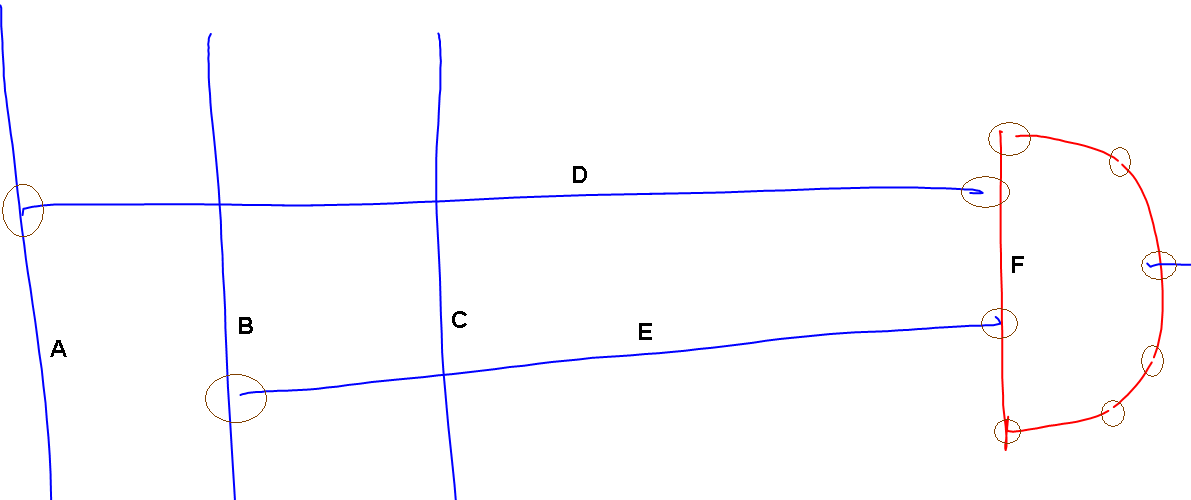
\includegraphics[width=3.0in]{adjacencies.png}%sample.eps}
\caption{Blue strokes are labeled ``WIRE'' and red strokes are labeled ``GATE''. 
Even though the wire and gate strokes are in their own component, we can still test whether or not the strokes are adjacent.}
\label{fig:adjacencies}
\end{figure}

A connectivity matrix is similar to an adjacency matrix, except it determines whether two strokes are connected (that is, there is a path between the two strokes).
To create the connection matrix, a depth first search is tried on all pairwise combinations of the strokes in the group.
Depth first search works by marking the current vertex as visited, and performing depth first search on all non visited neighboring vertices (found from the adjacency matrix).
This process repeats until it finds the goal, or it runs out of vertices to try.
Once the connectivity matrix has been created, it is simple to find the connected components.
The connected components are just those that have the same row entry.

\begin{figure}[h]
\centering
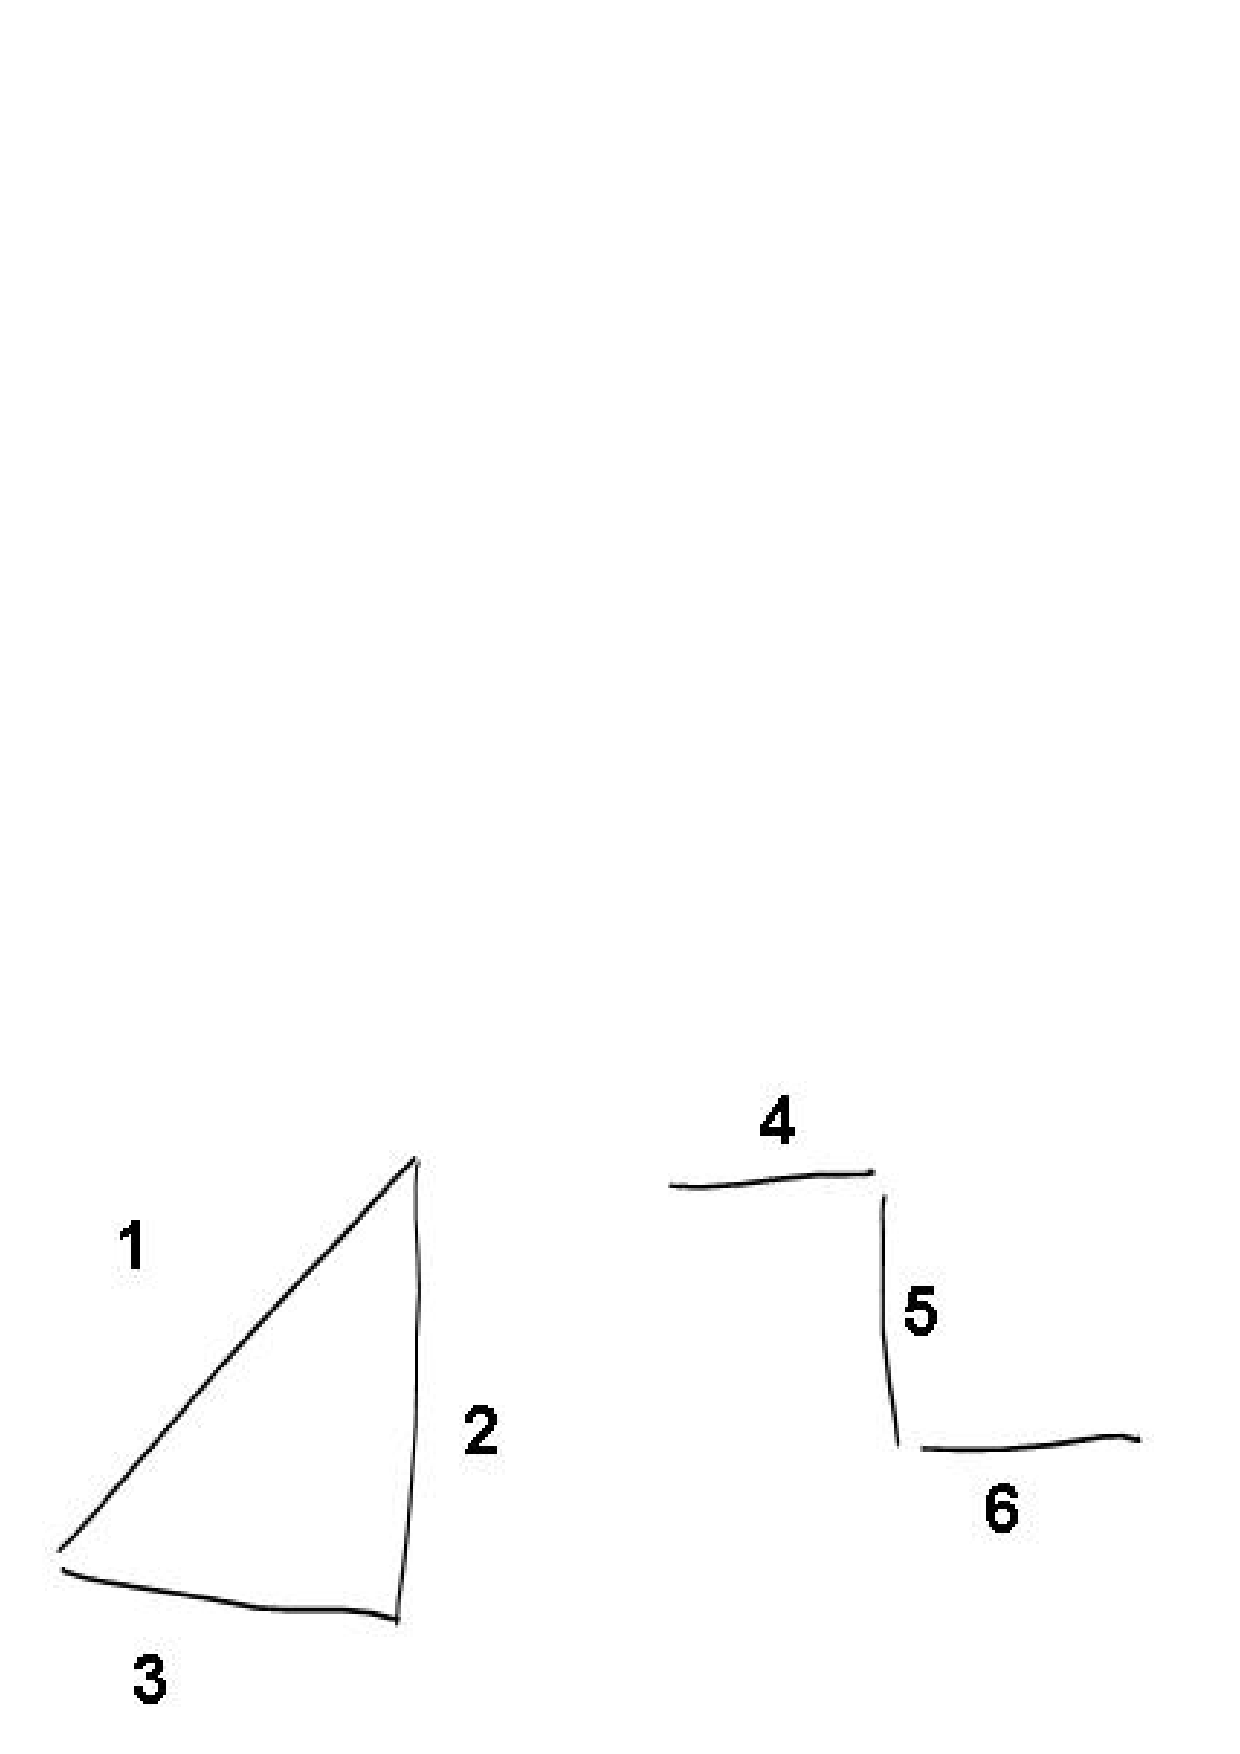
\includegraphics[width=3.0in]{connections.png}%sample.eps}
\caption{Strokes \{1 2 3\} compose a connected component as do strokes \{4 5 6\}.}
\label{fig:connections}
\end{figure}

For Figure~\ref{fig:connections}, an adjacency matrix would be
$$
\left(
\begin{array}{cccccc}
0&1&1&0&0&0\\
1&0&1&0&0&0\\
1&1&0&0&0&0\\
0&0&0&0&1&0\\
0&0&0&1&0&1\\
0&0&0&0&1&0\\
\end{array}
\right).
$$
A connection matrix would be
$$
\left(
\begin{array}{cccccc}
1&1&1&0&0&0\\
1&1&1&0&0&0\\
1&1&1&0&0&0\\
0&0&0&1&1&1\\
0&0&0&1&1&1\\
0&0&0&1&1&1\\
\end{array}
\right).
$$
Notice that rows 1, 2, and 3 are the same, and rows 4, 5, and 6 are the same, thus the connected components are \{\{1 2 3\} \{4 5 6\}\}.

\subsection{Update Partitioning}
Note: this section consists of proposed methods to update the partitioning.

After the initial segmentation into components, we can try to recognize all of the components with symbol recognition.
Updating the partition is done if every component has a probability greater than $\beta$.

Segmentation is not usually done after the initial segmentation though.
We can go through a series of single stroke corrections by adding and removing strokes from components, as well as creating or removing components to correct for errors in initial segmentation.
After a component has gone through symbol recognition, if the component is not recognized, then the probabilities of the labels of the strokes in the component will come into use.
The lowest probability may have its associated stroke removed from the component to see if symbol recognition increases.
Using similar techniques, this stroke can be added to other components to see if their symbol recognition increases.
If it does not help any of the other components, it may become its own component.
If removing the lowest probability stroke does not increase recognition, then the next lowest probability stroke can go through this same process.

After single strokes corrections have been made, multiple stroke corrections can be made.
Multiple stroke correction will break a single component into multiple components (thus will fix the initial segmentation overfitting).
Again, we could try every partition of the component, but in the pathological case we would be looking at a component that has too many strokes.
To speed up segmentation for a component that has been overfitted, we take into account the relative temporal ordering of the strokes.
Here we enforce that the any better fitting component inside the current component must be in absolute, strict order.
And to begin with, we are only trying to find a single component.
For example, consider the component with ordered strokes [1 2 3 4].
Using this method we would test the following: \{\{1\} \{2\} \{3\} \{4\} \{1 2\} \{2 3\} \{3 4\} \{1 2 3\} \{2 3 4\} \{1 2 3 4\}\} parts against the recognizer.
Assuming the recognizer takes constant time, this method takes $n(n+1)/2$ time, or $O(n^2)$ time where $n$ is the number of strokes to extract a better component.
Let us say that \{2 3\} gave us the best results.
Then \{2 3\} would be taken out of the previous component, and given its own component.
The previous component would then become \{1 4\}.
%We could test the previous component again for multiple stroke correction.
%Thus, it would be \{\{1\}, \{4\}, \{1 4\}\}.
%We keep repeating this process until the component does not change.
%In the worst case (which we would hope could never happen), we could remove a single stroke each iteration, and repeat the  process with $n - 1$ strokes.
%Thus, in the worst case, the process of correcting a single component for multiple strokes takes $O(n^3)$ time (Expected $O(n^2)$ or $O(n^2\log{n})$ I think...). 

After all the multiple stroke corrections have been made, we can repeat the cycle of single and multiple stroke correction again on all components.

In the case where these somewhat simplistic single and multiple stroke corrections do not achieve recognition of all components, other partitioning strategies may be employed. Such strategies may involve rehashing the adjacency and connection matrices within the components by making $\alpha$ more restrictive, thus modifying the condition for adjacency. Another method may involve a breadth first search around the initial partition.

\section{Results and Discussion}
The graph theory segmentation is not as complete as we would like it to be.
The main reason for this is due to the fact that we do not have a symbol based recognizer and updating the partitioning relies on a symbol recognition.
Initial segmentation is in a working state.

The data we tested against was collected from 17 individuals, each of whom drew 3 sketches.

In testing \emph{only} the performance of initial segmentation, segmentation was run on correct hand labeled data.
That way, we are not getting errors from anything but segmentation.
We tested the number of overfitted and underfitted components against the correct number of components and calculated the percentage of components that were correct.
An overfitting is putting multiple components into the same component, while underfitting is breaking up a single component into multiple components.
We also tested initial segmentation against the same data, but instead of being hand labeled, it was labeled with the labeling step.
Results for the hand labeled and labeling step data can be found in Table~\ref{table:results1}.

\begin{table}[h]
\begin{tabular}{|p{1.9cm}|p{2.1cm}p{1.5cm}p{1.6cm}|}
	\hline
Data Set 				&  Correctness(\%)		& Overfit(\%) 		& Underfit(\%)  \\
	\hline
Hand labeled   	& $88 \pm 2$					& $9 \pm 1$						& $2 \pm 1$ \\
Labeling step 	 	& $77 \pm 3$					& $16 \pm 3$			 & $6 \pm 1$ \\
	\hline
\end{tabular}
\caption{As expected, the hand labeled data set produces better results than the labeling step data set.  This is because the labeling step introduces some errors.}
\label{table:results1}
\end{table}

It seemed the biggest problem that initial segmentation has right now is dealing with wires.  
Even though there is a modified minimum distance measure for wires, it was not enough to stop the wires from becoming constantly overfitted.
As for gates, those that resulted in errors were underfit, and those were the gates that had circles at the end of them (such as ``NAND'', ``NOT'', and ``NOR'' gates).
The circles were either getting mislabeled in the labeling step, or were to far away from the other strokes in the gate.
In Table~\ref{table:results2} we have the composition of the errors.

\begin{table}[h]
\begin{tabular}{|cc|}
\hline
Wire (\%)& Gate (\%)\\
\hline
$80 \pm 1$ & $20 \pm 1$\\
\hline
\end{tabular}
\caption{The majority of errors were due to wires.}  
\label{table:results2}
\end{table}


\section{Related Work}

In~\cite{spatial} we see a similar graph theory method.
We have added on the idea of a component.

\section{Future Work}
There is still a lot of work needed to get segmentation working as we would like it.
The biggest part in this process is creating a symbol recognizer to work side by side with segmentation, like the recognizer presented in~\cite{zernike}.
There they present a symbol based recognizer using $n(n - 1)/2$ binary SVM classifiers with zernike moments as one of the features.
The only challenge would be translating the $n(n - 1)/2$ distances from the hyperplane into probabilities.
There are ways to achieve the measure of probability though.
For that, look into~\cite{ping-simple} and~\cite{roth01probabilistic}.

Another possibility for symbol recognition would be to train a Conditional Random Field (CRF) on just the symbols.
Even though the CRF labels each stroke, with such a small stroke count composing each symbol and ample training data, one would hope that the CRF would always apply the same label to all of the strokes.

It would also be worthwhile to research into how different adjacency measures effect the output of segmentation.
That would also include adjusting the thresholds to achieve the desired correctness of segmentation.
There are also some questions to be asked of the adjacency measure.
Should each label have its own adjacency measure like wires do now?
Can there be a common measure applied to all strokes?

While segmentation will tell you what group of strokes compose the different components, even that much in not considered full sketch recognition.
The final part of sketch recognition would be to figure out how everything interconnects.  
That is, figuring out that this wire that comes out of this gate connects to the back of that gate.
Full sketch recognition would be creating the corresponding truth table.

\section{Conclusion}
In this paper we have shown that segmentation, even with labeled data, is not a trivial problem.
In the pursuit of segmentation, the graph theory method has been shown as a way to initially partition a sketch (in polynomial $O(n^2)$? time).
Additional methods have been proposed to correct for single stroke errors and multiple stroke errors during the updating partition step.

\begin{figure}[h]
\centering
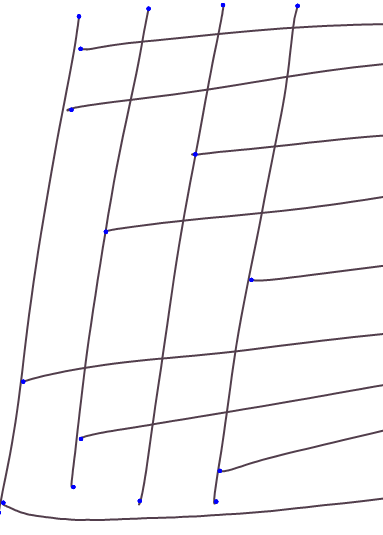
\includegraphics[width=1.0in]{missegmentedwire1.png}
\label{fig:connections}
\end{figure}

\begin{figure}[h]
\centering
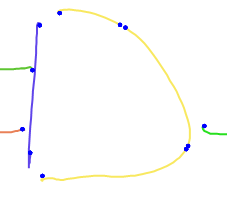
\includegraphics[width=1.0in]{missegmentedgate1.png}
\label{fig:connections}
\end{figure}

\begin{figure}[h]
\centering
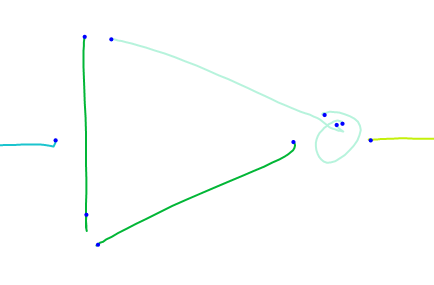
\includegraphics[width=1.0in]{missegmentedgate2.png}
\label{fig:connections}
\end{figure}

\begin{figure}[h]
\centering
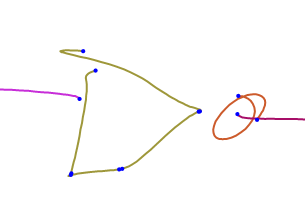
\includegraphics[width=1.0in]{missegmentedgate3.png}
\label{fig:connections}
\end{figure}

\bibliographystyle{acmsiggraph}
\nocite{*}
\bibliography{devin}
\end{document}
